\chapter{Evaluation}

\begin{figure}[b]
    \centering
    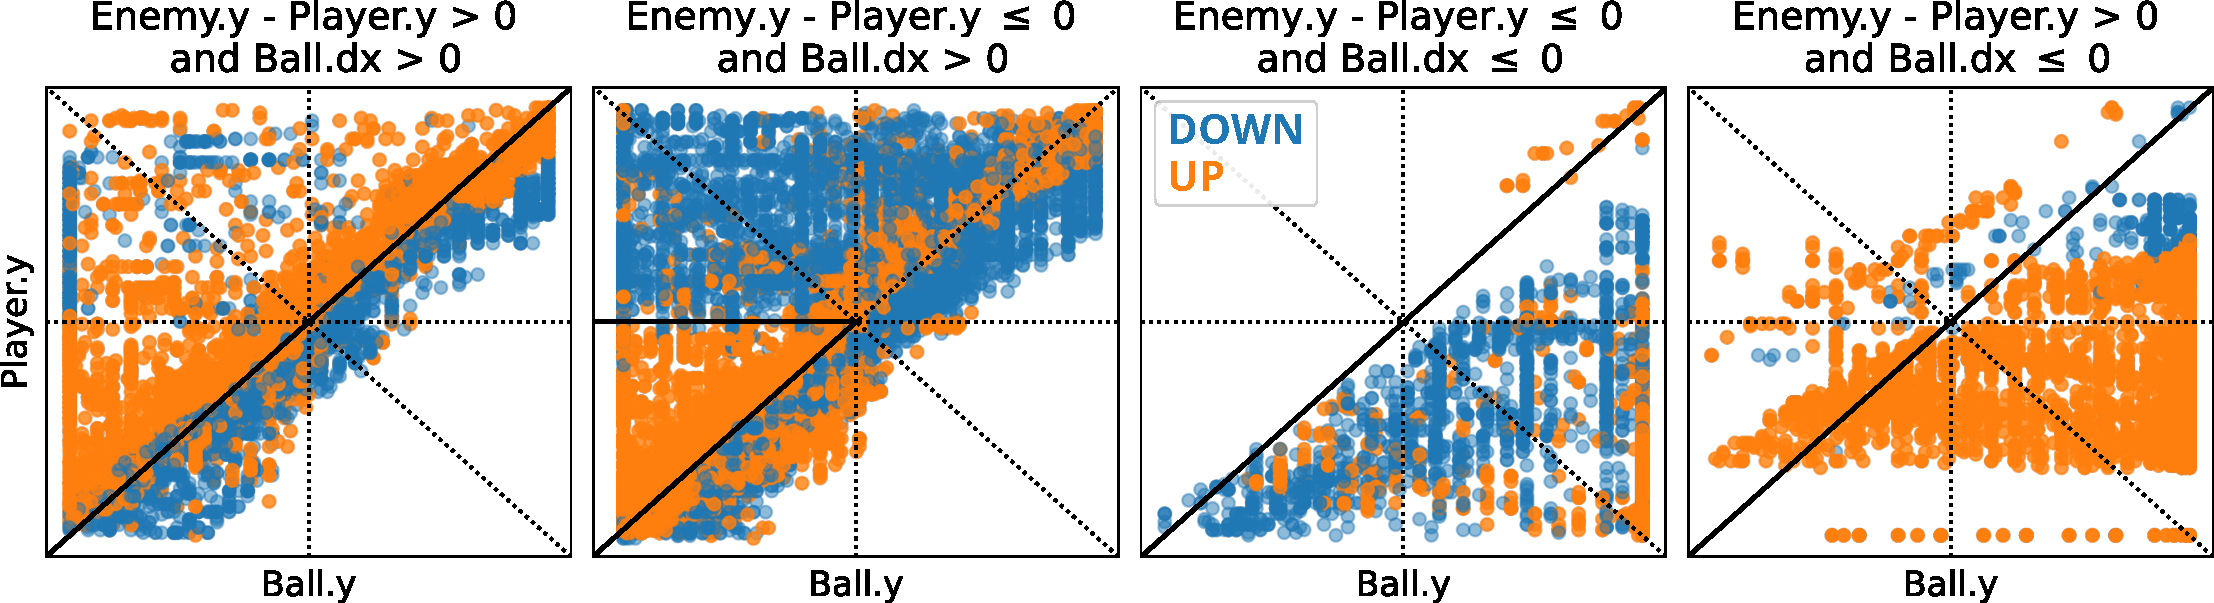
\includegraphics[width=1.\textwidth]{images/images_part3/pong_state_space.pdf}
    \caption{\textbf{Oracle decision rules are oblique} illustrated on PPO for different state space partitions of the Pong environment. Decisions boundaries are both oblique and parallel.}
    \label{fig:pong_states}
\end{figure}


\begin{figure}[b]
    \centering
    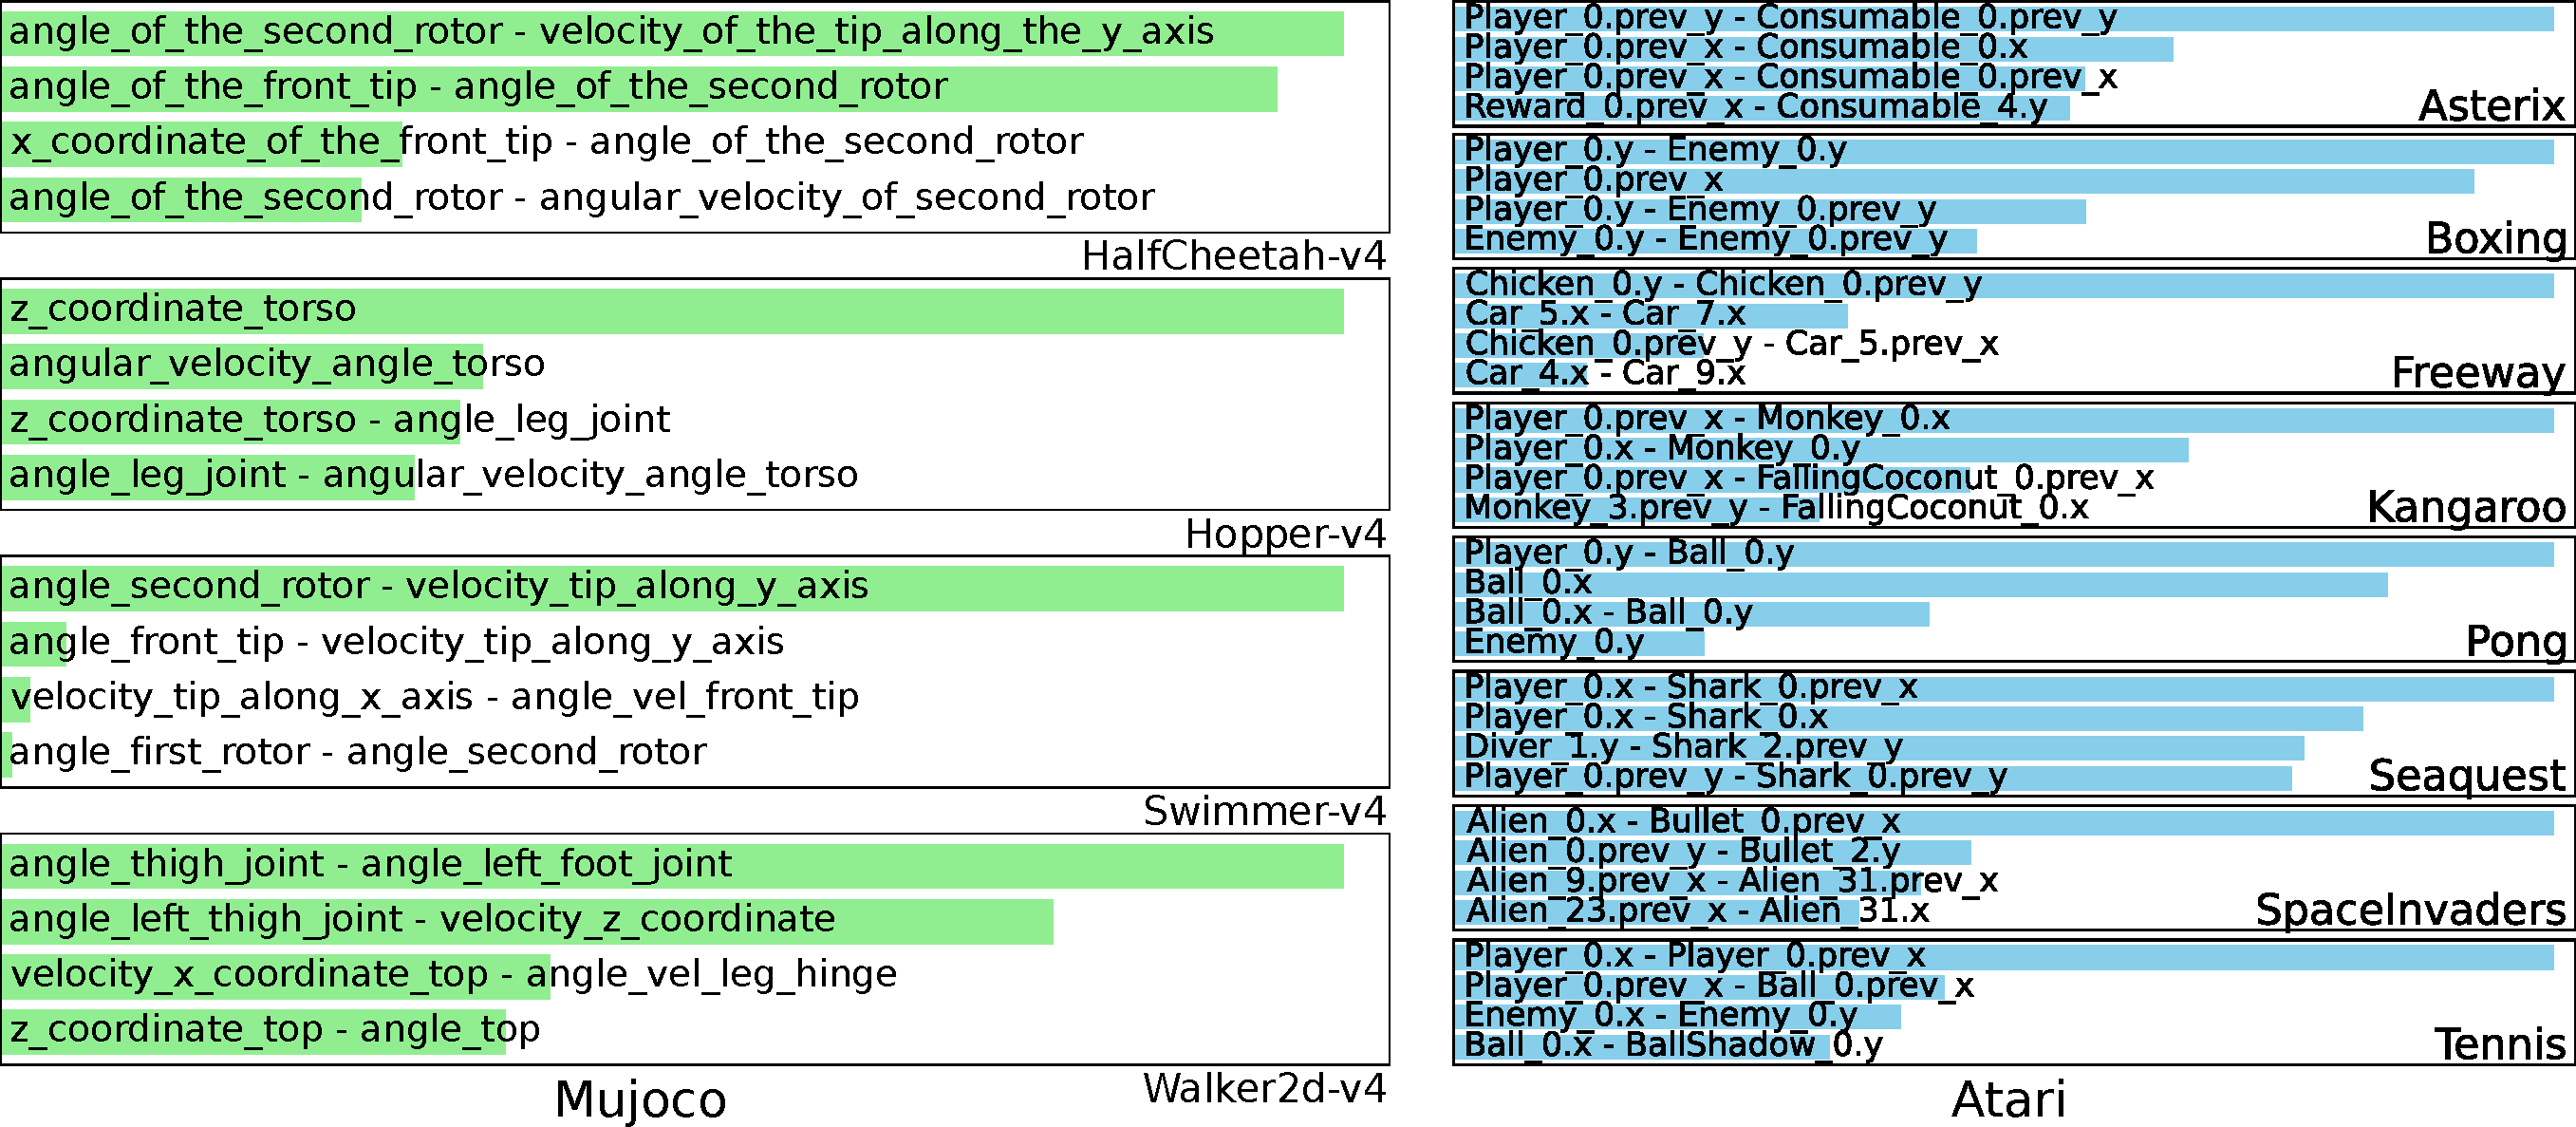
\includegraphics[width=1.\textwidth]{images/images_part3/dis_mujoco+f_atari.pdf}
    \caption{\textbf{Oracle decision rules are oblique} illustrated on PPO for different state space partitions of the Pong environment. Decisions boundaries are both oblique and parallel.}
    \label{fig:pong_states}
\end{figure}

\begin{figure}[b]
    \centering
    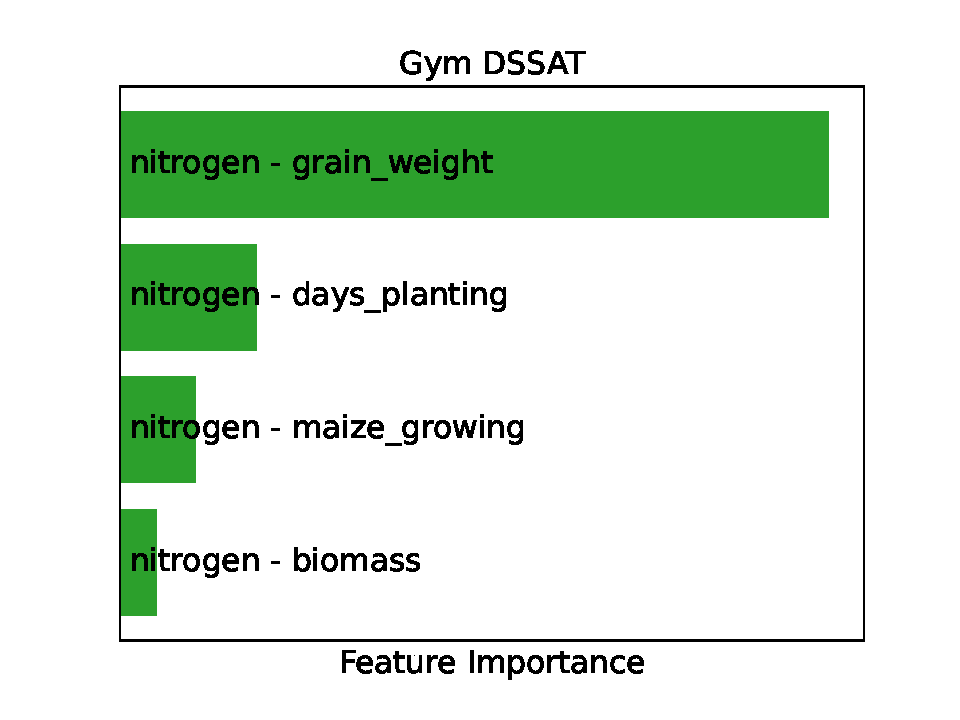
\includegraphics[width=1.\textwidth]{images/images_part3/fi_dssat_copy_human.pdf}
    \caption{\textbf{Oracle decision rules are oblique} illustrated on PPO for different state space partitions of the Pong environment. Decisions boundaries are both oblique and parallel.}
    \label{fig:pong_states}
\end{figure}

\textbf{Oblique decision trees.} One can imitate oracles with programs that make tests of linear combinations of features. Many oracles learn oblique or more complex decision rules over an MDP state space. This is illustrated in Figure~\ref{fig:pong_states} where a PPO neural oracle creates oblique partitions of the state-space for the Pong environments. Programs that test only individual features would fail to fit this partition (see Figure~\ref{fig:pong_states}). 
We thus modify CART~\citep{breiman}, an algorithm returning axes-parallel trees for regression and supervised classification problems, for it to return oblique decision trees. 

In addition to single feature tests, our oblique trees consider linear combinations of two features with weights $1$ and $-1$, e.g., for MDP states $s_i \in \mathbb{R}^{p}$, the oblique features values are $s^{oblique}_i = \{s_{i1} - s_{i0}, s_{i2} - s_{i0}, \ldots, s_{ip} - s_{i0}, \ldots, s_{ip-1} - s_{ip}\} \in \mathbb{R}^{p^2}$. For example, using an oracle dataset with $n$ state-actions pairs: $(\bar{S}, \bar{A} = \pi^{*}(\bar{S})) \subsetneq \mathbb{R}^{n\cdot(p+\dim(A))}$, we obtain oblique decision trees by fitting $(\bar{S},\bar{S}^{oblique} , \bar{A} = \pi^{*}(\bar{S})) \subsetneq \mathbb{R}^{n\cdot(p(p+1)+\dim(A))}$. 
Given $\bar{S}$, computing $\bar{S}^{oblique}$ can be done efficiently by computing the values of the lower (or upper) triangles in the $\bar{S} \otimes \bar{S} - (\bar{S} \otimes \bar{S})^T$ tensor (excluding the diagonals) (see line~\ref{alg:oblique2} of Algorithm~\ref{alg:iqdagger}). We further demonstrate the superiority of oblique trees in our experimental evaluation on a diverse set of RL tasks.

\begin{wraptable}[7]{r}{0.55\textwidth}
\centering
\vspace{-0.5mm}
\caption{ \textbf{\small Automated masking reduces the number of features in MDP}, illustrated on $8$ Atari environments.}
\setlength{\tabcolsep}{3pt}
\scalebox{0.9}{
\begin{tabular}{@{}ccccccccc@{}}
\toprule
MDP        & \small Ast. & Box. & \small Free. & \small Kang. & \small Pong & \small Sea. & \small SpaceI. & Ten. \\ \midrule
Full    & 100         & 8    & 48           & 196          & 12          & 172         & 176            & 16   \\
Simplified & 90          & 8    & 22           & 28           & 8           & 54          & 164            & 16   \\ \bottomrule
\end{tabular}}
\label{tab:repartitions}
\end{wraptable}

\textbf{The complexity} of building the tree (line \ref{alg:cart2} of algorithm \ref{alg:iqdagger}) is $O(pn\log_2(n))$ when no maximum tree depth is given, and $O(pnD)$ with a maximum tree depth of $D$ \citep{complexcart}. 
In particular, at iteration $i$ of our algorithm the complexity of building the tree is $O(p(p+1)itD)$, as rollouts of $t$ MDP transitions are aggregated (line \ref{alg:aggreg}) and oblique features are added to states (line \ref{alg:oblique2}). 
This means that at each iteration $i$, the cost of computing an oblique tree is $p+1$ times the cost of computing an axes-parallel tree. In our algorithm we pass $K$ the maximum number of leaf nodes as an argument. A tree with $K$ leaf nodes has $2K - 1$ total nodes and a depth of at most $D=K-1$.

\subsection{Real life use case of \interpreter tree programs for fertilization of soils (Q3)}
\begin{wrapfigure}[18]{r}{0.53\textwidth}
\centering
\vspace{-5.6mm}
\footnotesize
\inputminted{Python}{annexes/programmes/play_dssat_oblique_66.2_copy_human.py}
\caption{\textbf{\interpreter can explain human heuristic policies.} \interpreter program with 100\% accuracy on human oracle policy.}
\vspace{-2mm}
\label{fig:dssat-iqdagger}
\end{wrapfigure}
In this last experiment, we distill a human expert policy for soil fertilization on the \texttt{gym-DSSAT gym} environment \cite{gautron2023learning}. Here, an RL agent has to learn to manage a crop, based on an accurate simulated mechanistic model of plant growth. 
We consider the task that consists in optimizing plant nitrogen absorption while penalizing the application of fertilizer to minimize the economical and the environmental costs. 
We extract an \interpreter's Python program, depicted in Figure~\ref{fig:dssat-iqdagger}. 
This program outputs the exact same actions as the human heuristic given the soil state and obtain the same cumulative reward in average (corresponding to an accuracy of $100\%$). 
It also provides an interpretation of the human expert heuristic that delivers a certain amount of fertilizer ($\{27, 35, 54\}$) after $\{39, 45, 80\}$ days after seeding, respectively). 
The feature importance coincides with agronomic principles and have been validated by an expert from the \textit{Consultative Group on International Agricultural Research}. 
The nitrogen requirements of corn vary depending on the growth stage. They are important during the vegetative phase (plant growth) and the reproductive phase (from flowering to grain filling). This is why it is essential to consider the number of days after planting and the growth stage of the corn, as nitrogen requirements are highest during grain filling.

\section{Methodology Overview}\label{sec:methodology}
In this section, we explain our methodology for the evaluation of interpretability.
Our approach consists of three main steps: (1) obtaining deep neural network policies trained with reinforcement learning that obtain high cumulative rewards, (2) distilling those policies into less complex ones to use as baselines (3) after parsing baselines from different classes into a common comparable language, we evaluate the interpretability of the policies using proxy metrics for \textit{simulatability}.

\paragraph{Deep Neural Network Policies}
In reinforcement learning, an agent learns how to behave in an environment to maximize a cumulative reward signal~\cite{sutton}. 
The environment is defined by a Markov decision process (MDP) $M = ( \mathcal{S}, \mathcal{A}, T, R)$, where $\mathcal{S}$ is the state space, $\mathcal{A}$ is the action space, $T : \mathcal{S} \times \mathcal{A} \times \mathcal{S} \rightarrow [0, 1]$ is the state-transition function, $R : \mathcal{S} \times \mathcal{A} \times \mathcal{S} \rightarrow \mathbb{R}$ is the reward function.
At each time step $t$, an agent observes the current state $s_t$ and chooses an action $a_t$ according to its policy $\pi$.
The agent executes $a_t$, receives reward $r_t$, and observes the next state $s_{t+1}'$.
The goal is to find an optimal policy $\pi^*$ that maximizes the expected discounted future return: $\pi^* = \operatorname{argmax}_{\pi} Q^\pi (s, a) =\operatorname{argmax} \mathbb{E}[r+\gamma Q^\pi(s', a)]$, with $\gamma$ a discount factor in $[0,1)$. For large or continuous state spaces like the MDPs we consider in this work, MLPs are used to represent $Q^\pi$ or $\pi$.
While these MLPs can be trained efficiently to obtain high cumulative rewards~\cite{ppo,dqn}, they are too complex for interpretability considerations.

\begin{algorithm}
\caption{Imitate Expert~\cite{behavior-cloning,dagger,viper}}\label{alg:distill}
\KwIn{Expert policy $\pi^*$, MDP $M$, policy class $\Pi$, number of iterations $N$, total samples $S$, importance sampling flag $I$}
\KwOut{Fitted student policy $\hat{\pi}_i$}

% Initialize empty dataset and initial policy
Initialize dataset $\mathcal{D} \gets \emptyset$\;
Initialize $\hat{\pi}_1$ arbitrarily from $\Pi$\;

\For{$i \gets 1$ \KwTo $N$}{
    % Create mixed policy using expert and current policy
    \lIf{i = 1}{
    $\pi_i \gets \pi^*$\
    }
      \lElse{
        $\pi_i \gets \hat{\pi}_i$
      } \label{alg:expert-or-student}
    % Collect data using mixed policy
    Sample $S/N$ transitions from $M$ using $\pi_i$\;
    \lIf{$I$ is True}{
    $w(s) \gets V^{\pi*}(s) - \operatorname{min}_aQ^{\pi*}(s, a)$
    }
      \lElse{
        $w(s) \gets 1$
      }
    % Get expert actions for visited states
    Collect dataset $\mathcal{D}_i \gets \{ (s, \pi^*(s), w(s)) \}$ of states visited by $\pi_i$ and expert actions\;\label{alg:actions-expert}
    
    % Aggregate datasets
    $\mathcal{D} \gets \mathcal{D} \cup \mathcal{D}_i$\;
    
    % Train new policy
   Fit classifier/regressor $\hat{\pi}_{i+1}$ on $\mathcal{D}$\;\label{alg:fit}
}

\Return $\hat{\pi}_N$\;
\end{algorithm}

\paragraph{Distilling into Interpretable Policies}
To obtain interpretable policies, we distill the complex neural networks into simpler models using imitation learning, as described in Algorithm \ref{alg:distill}. This approach transforms the reinforcement learning task into a sequence of supervised learning problems.


Algorithm \ref{alg:distill} inputs an environment, that simulates taking steps in an MDP, an expert policy to imitate, also called a teacher, and an (interpretable) policy class to fit, also called student. The hyperparameters of Algorithm \ref{alg:distill} are: the number of times we fit a student policy, the total number of samples to be collected, and whether or not to use importance sampling. At each iteration of Algorithm \ref{alg:distill} the student policy is fitted to a dataset of states collected with the expert at iteration 1 or with the previously fitted student (see Line \ref{alg:expert-or-student}). The actions are always given by the expert (see Line \ref{alg:actions-expert}). When using importance sampling, the states are further re-weighted by the worst state-action value possible in the given state. When the number of iteration is 1, Algorithm \ref{alg:distill} is behavior cloning~\cite{behavior-cloning}. When we use importance sampling, Algorithm \ref{alg:distill} is $Q$-DAgger~\cite{viper}. In other cases, Algorithm \ref{alg:distill} is DAgger~\cite{dagger}.

\paragraph{Measuring Policy Interpretability}
After obtaining interpretable policy baselines using Algorithm \ref{alg:distill}, we use two metrics to evaluate policy interpretability without requiring human intervention. Those metrics are proxies for the notion of \textit{simulatability} from~\cite{mythos} that gives insights on how a human being would read a policy to understand how actions are inferred. In particular, \textit{simulatability} admits two sub-definitions. The first one is a measure of how difficult it is for a human to reproduce the computations of the policy to infer actions given states. The second one measures how difficult it is for a human to read through the entire policy. \cite{mythos} argues that this nuance is key when measuring interpretability because a tree is not read entirely to compute a single action and because there is no consensus on what is easier for a human to read between an MLP and a tree. 

\textit{1. Policy Inference Time:} to measure how a human would compute the action of a policy given a state at each environment step, we measure policy step inference time in seconds.

\textit{2. Policy Size:} to measure how easily a human can read the entire policy, we measure its size in bytes. While this correlates with inference time for MLPs and linear models, tree-based policies may have large sizes but quick inference because they do not traverse all decision paths at each step.

As these measurements depend on many technical details (programming language, the compiler if any, the operating system, versions of libraries, the hardware it is executed on, etc), to ensure fair comparisons, we translate all student policies into a simple representation that mimics how a human being "reads" a policy. We call this process of standardizing policies language ``unfolding''.
%we ``unfold'' all policies into a common sequential representation without hardware optimizations or vectorized operations, as humans process information sequentially.
In Figure \ref{lst:unfolded-linear}, \ref{lst:generic-linear}, and \ref{lst:policy_ll}, we present some unfolded policy programs. Other works have distilled neural networks into programs \cite{PIRL} or even directly learn programmatic policies \cite{pirl2} from scratch. However, those works directly consider programs as a policy class and could compare a generic program (not unfolded, with, e.g., while loops or array operations) to, e.g, a decision tree \cite{leap}. We will discuss later on the limitations of unfolding policies in the overall methodology.

\begin{figure}
\centering
\begin{minipage}{0.487\textwidth}
\begin{tcolorbox}
\begin{lstlisting}[language=Python]
import gymnasium as gym

env = gym.make("MountainCar")
s, _ = env.reset()
done = False
while not done:
    y0 = 0.969*s[0]-30.830*s[1]+0.575
    y1 = -0.205*s[0]+22.592*s[1]-0.63
    y2 = -0.763*s[0]+8.237*s[1]+0.054
    max_val = y0
    action = 0
    if y1 > max_val:
        max_val = y1
        action = 1
    if y2 > max_val:
        action = 2
    s, r, terminated, truncated, \
    infos = env.step(action)
    done = terminated or truncated
\end{lstlisting}
\end{tcolorbox}
\caption{Unfolded linear policy interacting with an environment.}\label{lst:unfolded-linear}
\end{minipage}
\hfill
\begin{minipage}{0.505\textwidth}
\begin{tcolorbox}
\begin{lstlisting}[language=Python]
def play(x):
    h_layer_0_0 = 1.238*x[0]+0.971*x[1]
                  +0.430*x[2]+0.933
    h_layer_0_0 = max(0, h_layer_0_0)
    h_layer_0_1 = -1.221*x[0]+1.001
                  *x[1]-0.423*x[2]
                  +0.475
    h_layer_0_1 = max(0, h_layer_0_1)
    h_layer_1_0 = -0.109*h_layer_0_0
                  -0.377*h_layer_0_1
                  +1.694
    h_layer_1_0 = max(0, h_layer_1_0)
    h_layer_1_1 = -3.024*h_layer_0_0
                  -1.421*h_layer_0_1
                  +1.530
    h_layer_1_1 = max(0, h_layer_1_1)

    h_layer_2_0 = -1.790*h_layer_1_0
                  +2.840*h_layer_1_1
                  +0.658
    y_0 = h_layer_2_0
    return [y_0]
\end{lstlisting}
\end{tcolorbox}
\caption{Tiny ReLU MLP for Pendulum.}\label{lst:generic-linear}
\end{minipage}
\end{figure}

\begin{figure}
\centering
\begin{minipage}{0.545\textwidth}
\begin{tcolorbox}
\begin{lstlisting}[language=Python]
def play(x):
    if (x[3] - x[4]) <= -0.152:
        if (x[2] - x[3]) <= 0.049:
            return 3
        else:
            if x[5] <= 0.030:
                return 2
            else:
                if (x[2] - x[4]) <= 0.061:
                    return 3
                else:
                    #Fire main engine
                    return 2
    else:
        if (x[0] - x[6]) <= -0.840:
            return 0
        else:
            if (x[0] - x[4]) <= -0.007:
                # Fire right engine
                return 3
            else:
                # Fire left engine
                return 1
\end{lstlisting}
\end{tcolorbox}
\end{minipage}
\hfill
\begin{minipage}{0.43\textwidth}
    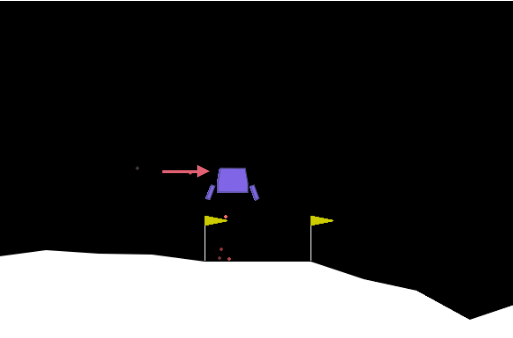
\includegraphics[trim={0 0 0 0},clip,scale=0.24]{images/images_part3/ll_d.png}
    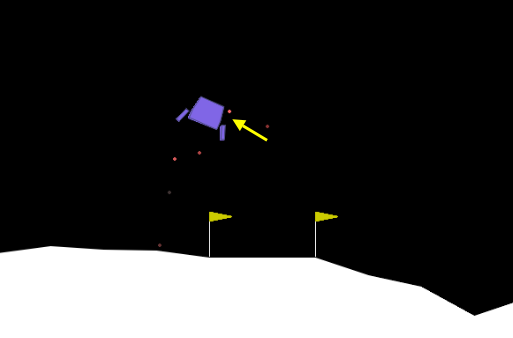
\includegraphics[scale=0.24]{images/images_part3/ll_b.png}
    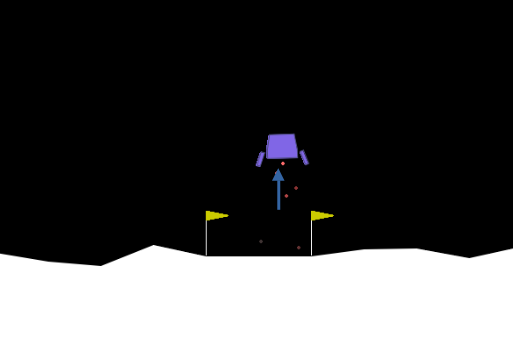
\includegraphics[trim={0 00cm 0 0},clip,scale=0.24]{images/images_part3/ll_g.png}
\end{minipage}
\caption{An unfolded oblique tree policy's actions obtaining 250 rewards on Lunar Lander.}\label{lst:policy_ll}
\end{figure}

\section{Computing Baseline Policies}

\subsection{Setup}
All the experiments presented next run on a dedicated cluster of Intel Xeon Gold 6130 (Skylake-SP), 2.10GHz, 2 CPUs/node, 16 cores/CPU with a timeout of 4 hours per experiment. Codes to reproduce our results are given in the supplementary material. In the future, we will open source a python library with all the tools of our methodology.
Using Algorithm \ref{alg:distill}, we distill deep neural network expert policies into less complex policy classes.

\paragraph{Policy classes}

\begin{table}[ht]
\centering
\small
\begin{tabular}{lll}
\hline
\textbf{Policy Class} & \textbf{Parameters} & \textbf{Training Algorithm} \\
\hline
Linear Policies & Determined by state-action dimensions & Linear/Logistic Regression \\
Decision Trees & [4, 8, 16, 64, 128] nodes & CART ($2\times$ nodes maximum leaves) \\
Oblique Decision Trees & [4, 8, 16, 64, 128] nodes & CART ($2\times$ nodes maximum leaves) \\
ReLU MLPs & [2$\times$2, 4$\times$4, 8$\times$8, 16$\times$16] weigths & Adam optimization (500 iterations) \\
\hline
\end{tabular}
\caption{Summary of baseline policy classes parameters and fitting algorithms (used in Line \ref{alg:fit}).}
\label{tab:policy-classes}
\end{table}

 We consider four policy classes for our baselines. We choose those policy classes because there exist efficient algorithms to fit them with supervised data which is a required step of imitation learning in Line \ref{alg:fit}. We consider linear policies that have been shown to be able to solve Mujoco tasks~\cite{empirical-evidence}. We fit linear policies to expert policies using simple linear (logistic) regressions with scikit-learn~\cite{scikit-learn} default implementation. We also consider decision trees~\cite{cart} and oblique decision trees~\cite{oblique}. (Oblique) Decision trees are often considered the most interpretable model class in machine learning~\cite{mythos} and reinforcement learning~\cite{viper,IBMDP,glanois-survey,milani-survey}. We train trees using the default CART~\cite{cart} implementation of scikit-learn with varying numbers of parameters (number of nodes in the tree). We also consider MLPs with ReLU activations~\cite{relunet} with varying number of parameters (total number of weights). This class of policy is often considered the least interpretable and is often used in deep reinforcement learning~\cite{deep-rl-relu1,deep-rl-relu2,deep-rl-relu3}. We train ReLU MLPs using the default scikit-learn implementation of Adam optimization~\cite{adam} with 500 iterations. The 15 baseline policy classes that we consider are summarized in Appendix \ref{tab:policy-classes}. 
\paragraph{Neural network experts}
We do not train new deep reinforcement learning agents \cite{dqn,ppo,deep-rl-relu1} but rather re-use ones available at the stables-baselines3 zoo \cite{zoo}. Depending on the environments described next, we choose neural network policies from different deep reinforcement learning agents. Some may argue that during the imitation learning, ReLU MLPs baselines may obtain better performance because they are often from the same class as the expert they imitate unlike trees. But this is not of our concern as we do not benchmark the imitation learning algorithms. Furthermore, it is important to note that not all experts are compatible with all the variants of imitation learning Algorithm \ref{alg:distill}. Indeed, SAC experts \cite{deep-rl-relu1} are not compatible with $Q$-DAgger \cite{viper} because it only works for continuous actions; and PPO experts, despite working with discrete actions do not compute a $Q$-function necessary for the re-weighting in $Q$-DAgger.

\paragraph{Environments}
We consider common environments in reinforcement learning research. We consider the classic control tasks from gymnasium \cite{gymnasium}, MuJoCo robots from \cite{mujoco}, and Atari games from \cite{atari}. For Atari games, since the state space is frame pixels that can't be interpreted, we use the object-centric version of the games from \cite{ocatari}. In Appendix \ref{tab:envs} we give the list of environments we consider in our experiments with their state-action spaces as well as a cumulative reward threshold past which an environment is consider ``solved''.

\subsection{Ablation study of imitation learning}\label{sec:res-imit}

In this section, we present the results of the expert distillation into smaller policies. For each environment, we fit all the policy classes. To do so, we run different instantiations of Algorithm \ref{alg:distill} multiple times with different total sample sizes. For each environment and each imitation learning variant, we summarize the number of times we fit all the baselines to an expert and which expert we use. The number of runs and imitation algorithm variants of Algorithm \ref{alg:distill} are summarized in Appendix \ref{tab:repet-distill}. After running the imitation learnings, we obtain roughly 40000 baseline policies (35000 for classic control, 5000 thousands for MuJoCo and 400 for OCAtari). A dataset with all the baselines measurements is given in the supplementary material.

\begin{figure}[ht]
\centering
\begin{subfigure}{.33\textwidth}
  \centering
  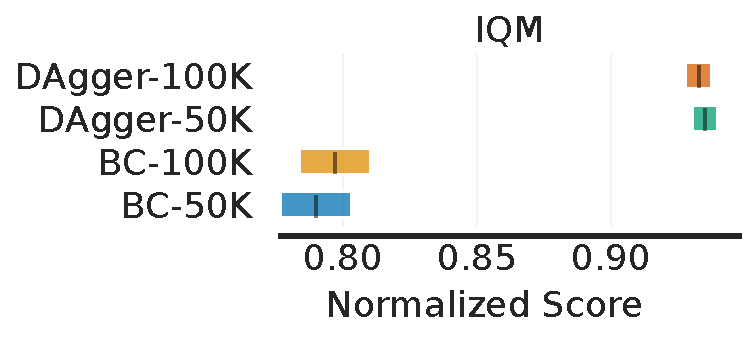
\includegraphics[width=\linewidth]{images/images_part3/ppo_expert_classic_control.pdf}
  \caption{Classic control, PPO expert}
  \label{fig:ppo_classic}
\end{subfigure}%
\begin{subfigure}{.33\textwidth}
  \centering
  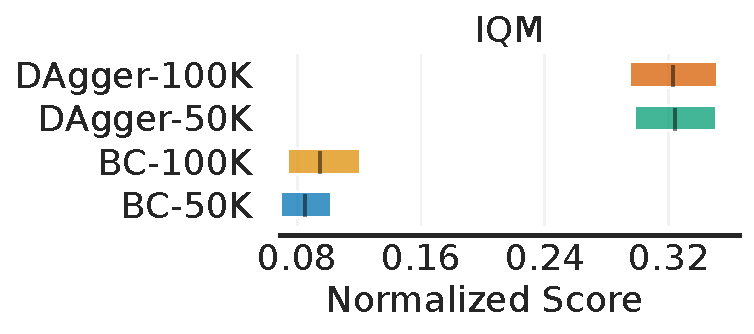
\includegraphics[width=\linewidth]{images/images_part3/sac_expert_mujoco.pdf}
  \caption{MuJoCo, SAC expert}
  \label{fig:sac_mujoco}
\end{subfigure}
\begin{subfigure}{.33\textwidth}
  \centering
  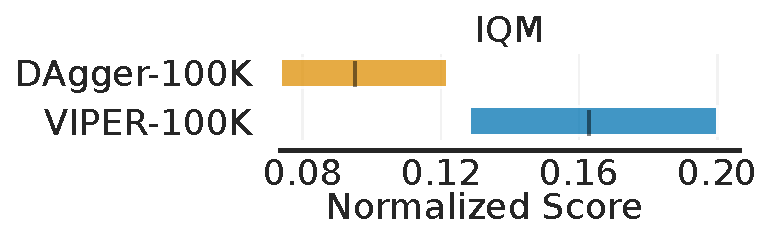
\includegraphics[width=\linewidth]{images/images_part3/dqn_expert_atari.pdf}
  \caption{OCAtari, DQN expert}
  \label{fig:dqn_atari}
\end{subfigure}%
\caption{Performance of imitation learning variants of Algorithm \ref{alg:distill} on different environments. We plot the 95\% stratified bootstrapped confidence intervals around the IQMs.}
\label{fig:performance_comparison}
\end{figure}

\paragraph{What is the best imitation algorithm?}
Even though the focus of our work is to evaluate trained policies, we still provide some insights on the best way to obtain interpretable policies from experts. Using the reinforcement learning evaluation library rliable~\cite{rliable}, we plot on Figure \ref{fig:performance_comparison} the interquartile means (IQM, an estimator of the mean robust to outliers) of the baseline policies cumulative rewards averaged over 100 episodes. For each imitation algorithm variant, we aggregate cumulative rewards over environments and policy classes. We normalize the baselines cumulative rewards between expert and random agent cumulative rewards.

The key observation is that for tested environments (Figures \ref{fig:ppo_classic},\ref{fig:sac_mujoco}), Behavior Cloning is not an efficient way to train baseline policies compared to DAgger. This is probably because Behavior Cloning trains a student policy to match the expert's actions on states visited by the expert while DAgger trains a student to take the expert's actions on the states visited by the student~\cite{dagger}. An other observation is that the best performing imitation algorithms for MuJoCo (DAgger, Figure \ref{fig:sac_mujoco}) and OCAtari ($Q$-Dagger, Figure \ref{fig:dqn_atari}) obtain baselines that in average cannot match well the performances of the experts. However baseline policies almost always match the expert on simple tasks like classic control (Figure \ref{fig:ppo_classic}).

\paragraph{What is the best policy class in terms of reward?}

\begin{figure}[ht]
    \centering
    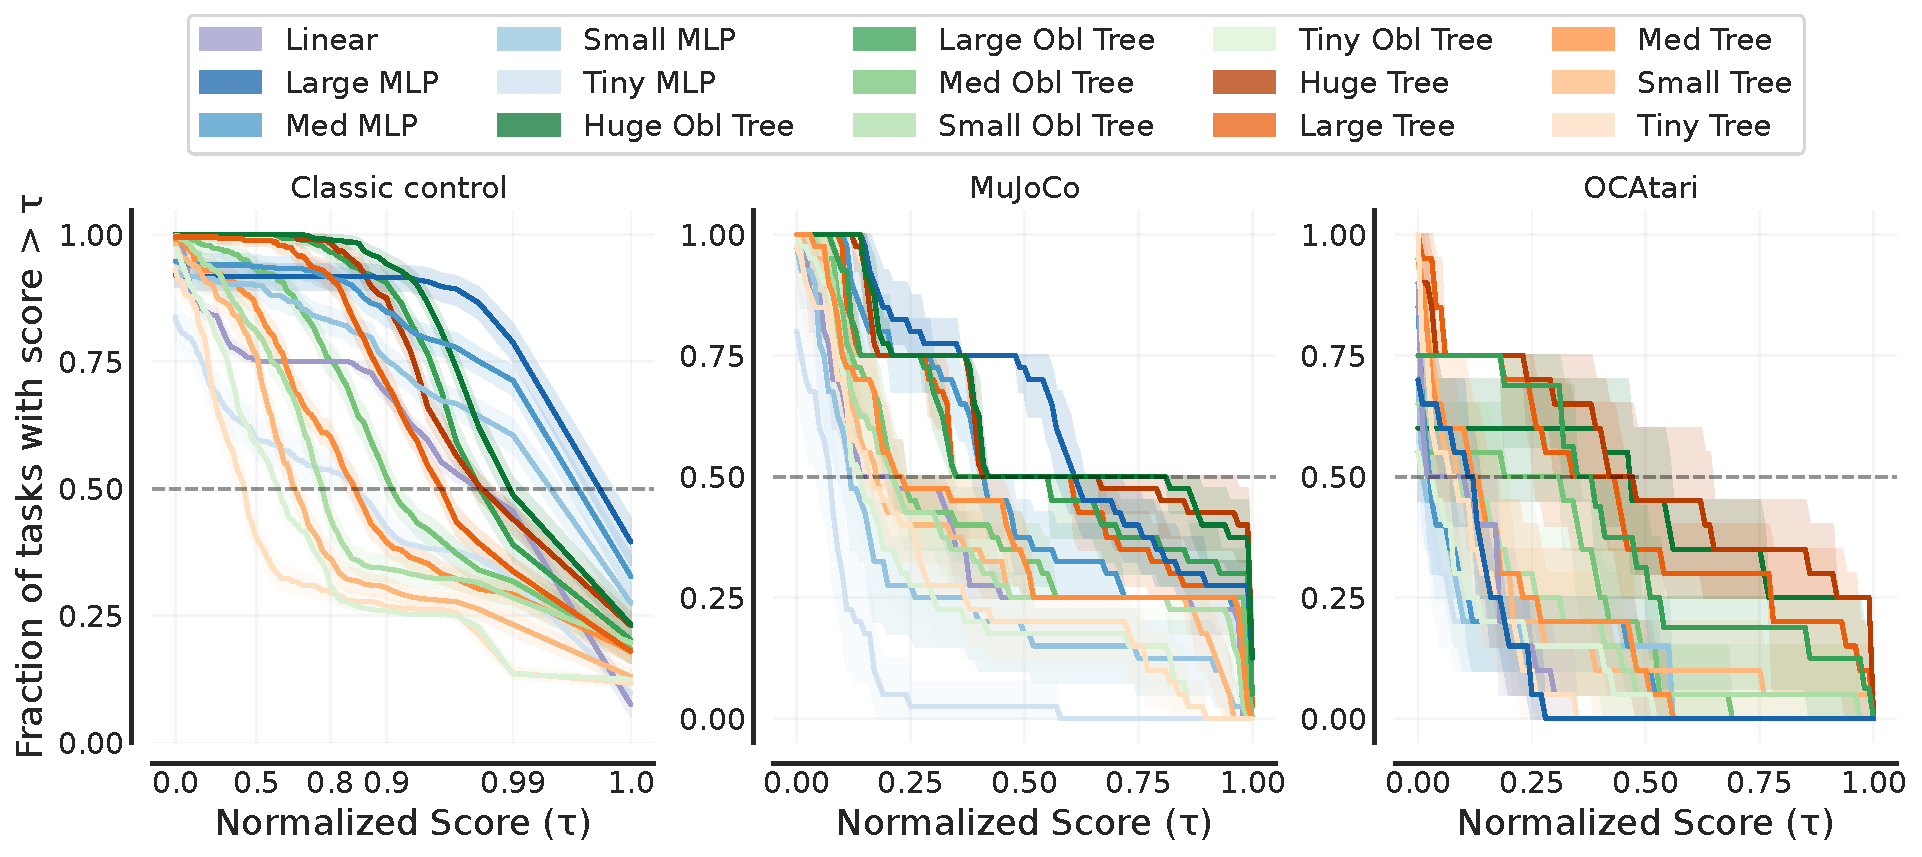
\includegraphics[trim={0 0 0 0.2cm},clip,width=0.9\linewidth]{images/images_part3/perf_profile_combined_100k.pdf}
    \caption{Performance profiles of different policy classes on different environments.}
    \label{fig:perf-combined}
\end{figure}

We also wonder if there is a policy class that matches expert performances more often than others across environments. For that we plot performance profiles of the different policy classes obtained with a fixed expert and fixed imitation learning algorithm. In particular, for each environments group we use the baseline policies obtained from the best performing imitation learning algorithm from Figure \ref{fig:performance_comparison}. From Figure \ref{fig:perf-combined} we see that on classic control environments, MLPs tend to perform better than other classes while on OCAtari games, trees tend to perform better than other classes. Now we move on to interpretability evaluation of our programmatic policies.



\section{Measuring Policy Interpretability}\label{sec:ablation-metric}
\subsection{From Policy to Program}
\begin{figure}
    \centering
    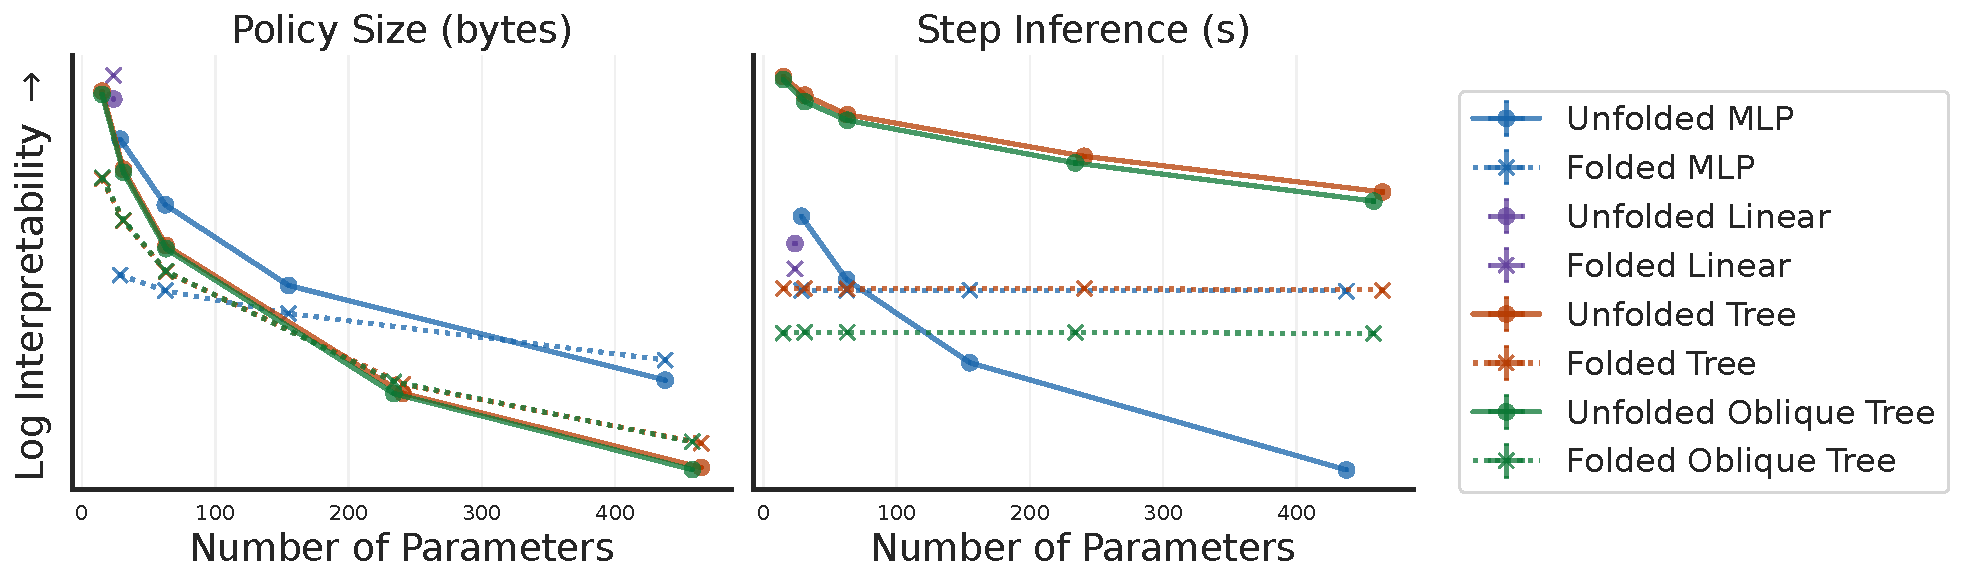
\includegraphics[width=1\linewidth]{images/images_part3/tree_sizes_memory_ppo_ci_ablation.pdf}
    \caption{Policies interpretability on classic control environments. We plot 95\% stratified bootstrapped confidence intervals around means in both axes. In each sub-plot, interpreatbility is measured with either bytes or inference speed.}
    \label{fig:abl-proxies}
\end{figure}

In this section, we compute the step inference times, as well as the policy size for both the folded and unfolded variant of each policy obtained for classic control environments with DAgger-100K. To unfold policies, we convert them into Python programs formatted with PEP 8 (comparing other unfolding formats such as ONNX \url{https://github.com/onnx/onnx} is left to future work). We ensure that all policies operations are performed sequentially and compute the metrics for each policy on 100 episodes using the same CPUs.

\paragraph{Is it necessary to unfold policies to compute interpretability metrics?} We see on Figure \ref{fig:abl-proxies} that folded policies of the same class almost always give similar interpretability values (dotted lines) despite having very different number of parameters. Hence, measuring folded policies interpretability would contradict established results from user studies such as, e.g., trees of different sizes have different levels of interpretability~\cite{study-4}. 

\paragraph{Is there a best policy class in terms of interpretability?}
User studies from~\cite{study-1,study-2,study-3} show that decision trees are easier to understand than models involving mathematical equations like oblique trees, linear maps, and MLPs. However,~\cite{mythos} states that for a human wanting to have a global idea of the inference of a policy, a compact MLP can be more interpretable than a very deep decision tree. In Figure \ref{fig:abl-proxies}, we show that inference speed and memory size of programs help us capture those nuances: policy interpretability does not only depend on the policy class but also on the metric choice. Indeed, when we measure interpretability with inference times, we do observe that trees are more interpretable than MLPs. However, when measuring interpretability with policy size, we observe that MLPs can be more interpretable than trees for similar number of parameters. Because there seem to not be a more interpretable policy class across proxy metrics, we will keep studying both metrics at the same time.




\subsection{Interpretability-performance trade-offs}\label{sec:res-trade-offs}

Now that we trained baseline policies and validated the proposed methodology, we use the latter to tackle open problems in interpretable reinforcement learning. For each environment, we fix the imitation learning algorithm and save the best baseline policy of each class in terms of episodic rewards after unfolding them. Each single Python policy is then \textbf{run again on the same dedicated CPU} for 100 new environment episodes (similarly to choosing a classifier with validation score and reporting the test score in the context of supervised learning).
\begin{figure}
    \centering
    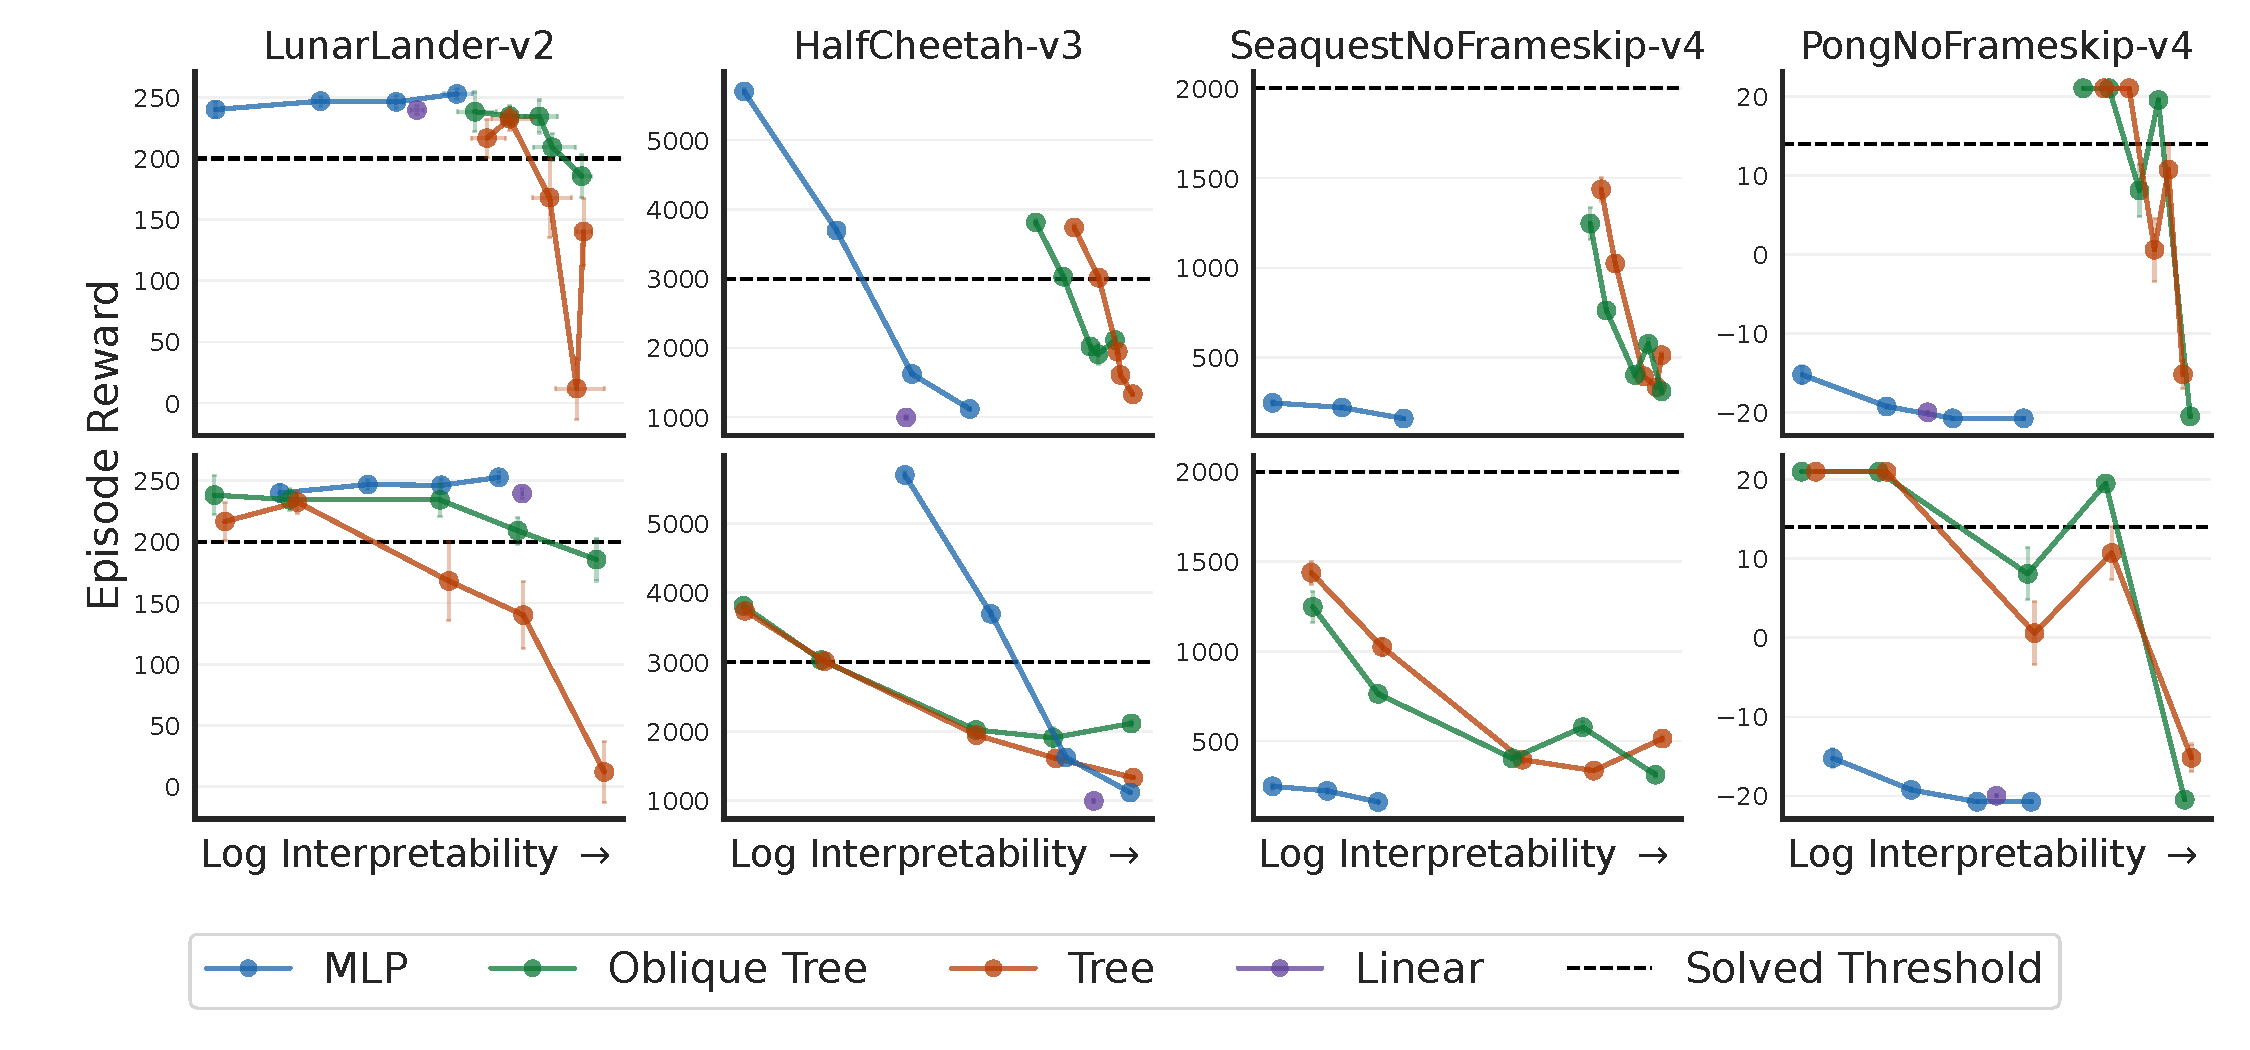
\includegraphics[trim={1.4cm 0 0 0},clip,width=1\textwidth]{images/images_part3/trade_off_select_combine_one_plot.pdf}
    \caption{Interpretabality-Performance trade-offs. Top row, interpretability is measured with step inference times. Bottom row, the interpretability is measured with policy size. We plot 95\% bootstrapped confidence intervals around means on both axes.}
    \label{fig:trade-off-summary}
\end{figure}

\paragraph{Is it possible to compute interpretable policies for high-dimensional environments?} \cite{glanois-survey} claim that computing an interpretable policy for high dimensional MDPs is difficult since it is similar to program synthesis which is known to be NP-hard \cite{program-synth}. Using our measures of interpretability, we can corroborate this claim. On Figure \ref{fig:trade-off-summary}, we can indeed observe that some relatively interpretable policies can solve Pong (20 state dimensions) or HalfCheetah (17 state dimensions) while for very high-dimensional environments like Seaquest (180 state dimensions), no baseline can solve the game.


\paragraph{For what environment are there good interpretable policies?}
We fitted a random forest regressor \cite{random} to predict the interpretability values of our baseline policies using environment attributes. In Table \ref{tab:combined_importance} we report the importance of each environment attribute when it comes to accurately predicting interpretability scores. We show that as hinted previously, the states dimensions of the environment is determining to predict the interpretability of good policies. Unsurprisingly, expert attributes also influence interpretability: for the environments where there is a positive large gap between expert and threshold rewards, the task could be considered easy and vice-versa.

\begin{table}
\centering
\small
\begin{tabular}{lcc}
\toprule
Environment Attributes & Importance for Step inference & Importance for Policy size \\
\midrule
States dimension & \textbf{80.87} & \textbf{35.52} \\
Expert episodes lengths & 11.39 & 9.28 \\
Episode reward of random & 2.26 & 4.75 \\
Expert episode reward & 1.51 & 16.80 \\
Episode reward to solve & 1.41 & 14.26 \\
Actions dimension & 1.41 & 2.02 \\
Expert reward - Solve reward & 1.15 & 17.37 \\
\bottomrule
\end{tabular}
\caption{Environment attributes importance to predict interpretability using either of our metrics.}
\label{tab:combined_importance}
\end{table}

\paragraph{How does interpretability influence performance?}
\cite{empirical-evidence,theory1} show the existence of linear and tree policies respectively that solve MuJoCo and continuous maze environments respectively; essentially showing that there exist environments for which policies more interpretable than deep neural networks can still compete performance-wise. Our evaluation indeed shows the existence of such environments. On Figure \ref{fig:trade-off-summary} we observe that on, e.g., 
LunarLander, increasing policy interpretability up to a certain point does not decrease reward. Actually, we can observe that for Pong a minimum level of interpretability is required to solve the game. Indeed, as stated in \cite{study-0}, optimizing interpretability can also be seen as regularizing the policy which can increase generalization capabilities. 
The key observation is that the policy class achieving the best interpretability-performance trade-off depends on the problem. Indeed, independent of the interpretability proxy metric, we see on Figure \ref{fig:trade-off-summary} that for LunarLander it is an MLP that achieves the best trade-off while for Pong it is a tree. Next, we compare our proxies for interpretability with another one; the verification time of policies used in \cite{viper,lens-complexity}.


\subsection{Verifying interpretable policies}
\cite{lens-complexity} states that the cost of formally verifying properties of MLPs scales exponentially with the number of the parameters. Hence, they propose to measure interpretability of a policy as the computations required to verify properties of actions given state subspaces, what they call local explainability queries \cite{query}. Before \cite{lens-complexity}, \cite{viper} also compared the time to formally verified properties of trees to the time to verify properties of MLPs to evaluate interpretability. In practice, this amounts to passing states and actions bounds and solving the SAT problem of finding a state in the state bounds for which the policy outputs an action in the action bounds. For example, for the LunarLander problem, a query could be to verify if when the y-position of the lander is below some threshold value, i.e, when the lander is close to the ground, there exists a state such that the tested policy would output the action of pushing towards the ground: if the solver outputs ``SAT'', then there is a risk that the lander crashes. 

Designing interesting queries covering all risks is an open problem, hence to evaluate the verification times of our baseline policies, we generate 500 random queries per environment by sampling state and action subspaces uniformily. Out of those queries we only report the verification times of ``UNSAT'' queries since to verify that, e.g., the lander does not crash we want the queries mentioned above to be ``UNSAT''. We also only verify instances of ReLU MLPs using \cite{maraboupy} for this experiment as verifying decision trees requires a different software \cite{z3} for which verification times would not be comparable.
\begin{figure}[ht]
    \centering
    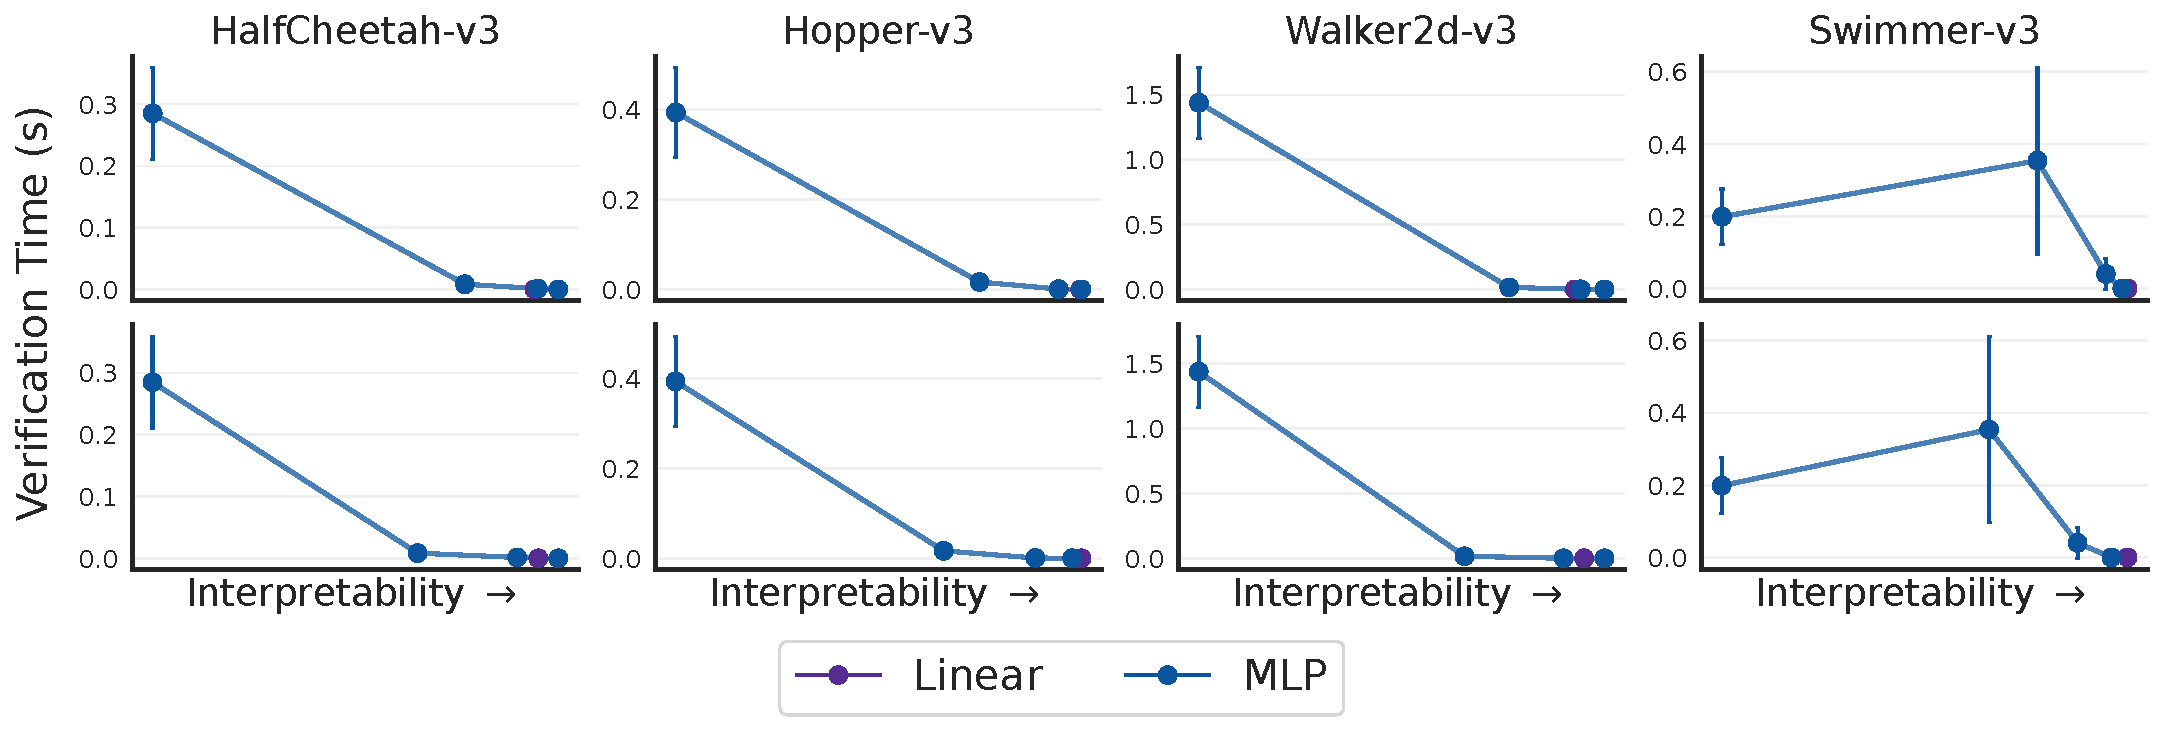
\includegraphics[width=1\linewidth]{images/images_part3/verification_tradeoff.pdf}
    \caption{Verification time as a function of policy interpretability. Top row, interpretability is measured with step inference times. Bottom row, the interpretability is measured with policy size. We plot 95\% confidence intervals around means on both axes.}
    \label{fig:trade-off-verif}
\end{figure}

On Figure \ref{fig:trade-off-verif}, we can observe that verification time decreases exponentially with MLP interpretability, both memory and inference speed, as shown in \cite{lens-complexity}. This is another good validation of our proposed methodology as well as a motivation to learn interpretable policies. 

\section{Experimental details}

In this section we give all the experimental details necessary to reproduce our results.



\begin{table}[ht]
\centering
\small
\begin{tabular}{lll}
\hline
\textbf{Classic} & \textbf{MuJoCo} & \textbf{OCAtari}\\
\hline
CartPole (4, 2, \textbf{490}) & Swimmer (8, 2, \textbf{300}) & Breakout (452, 4, \textbf{30})\\
LunarLander (8, 4, \textbf{200}) & Walker2d (17, 6, \textbf{2000}) & Pong (20, 6, \textbf{14})\\
LunarLanderContinuous (8, 2, \textbf{200}) & HalfCheetah (17, 6, \textbf{3000}) & SpaceInvaders (188, 6, \textbf{680})\\
BipedalWalker (24, 4, \textbf{250}) & Hopper (11, 3, \textbf{2000}) & Seaquest (180, 18, \textbf{2000})\\
MountainCar (2, 3, \textbf{90}) & \\
MountainCarContinuous (2, 1, \textbf{-110}) & \\
Acrobot (6, 3, \textbf{-100}) & \\
Pendulum (3, 1, \textbf{-400}) & \\
\hline
\end{tabular}
\caption{Summary of considered environments (dimensions of states and number or dimensions of actions, \textbf{reward thresholds}). The rewards thresholds are obtained from gymnasium \cite{gymnasium}. For OCAtari environments, we choose the thresholds as the minimum between the DQN expert from \cite{zoo} and the human scores. We also adapt subjectively some thresholds that we find too restrictive especially for MuJoCo (for example, the PPO expert from \cite{zoo} has 2200 reward on Hopper while the default threshold was 3800).}
\label{tab:envs}
\end{table}

\begin{table}
    \centering
    \footnotesize
    \begin{tabular}{c|cccccc}
    \toprule
    Envs & BC & BC & DAgger & DAgger & $Q$ & $Q$-DAgger\\
     & 50K & 100K & 50K & 100K & 50K & 100K\\
    \midrule
    Classic& 50 (PPO, DQN)& 50 (PPO, DQN)& 50 (PPO, DQN)& 50 (PPO, DQN)&  50 (DQN) & 50 (DQN)\\
    OCAtari& 0 & 0 & 0 & 5 (DQN)&  0 & 5 (DQN)\\
    Mujoco& 10 (SAC)& 10 (SAC)& 10 (SAC)& 10 (SAC)&  0 & 0\\
    \bottomrule
    \end{tabular}
    \caption{Repetitions of each imitation learning algorithm on each environment. We specify which deep reinforcement learning agent from the zoo~\cite{zoo} uses as experts in parentheses.}
    \label{tab:repet-distill}
\end{table}

\section{All interpretability-performance trade-offs}
In this appendix we provide the interpretability-performance trade-offs of all the tested environments. All the measures come from the experiment from Section \ref{sec:res-trade-offs}.

\begin{figure}
    \centering
    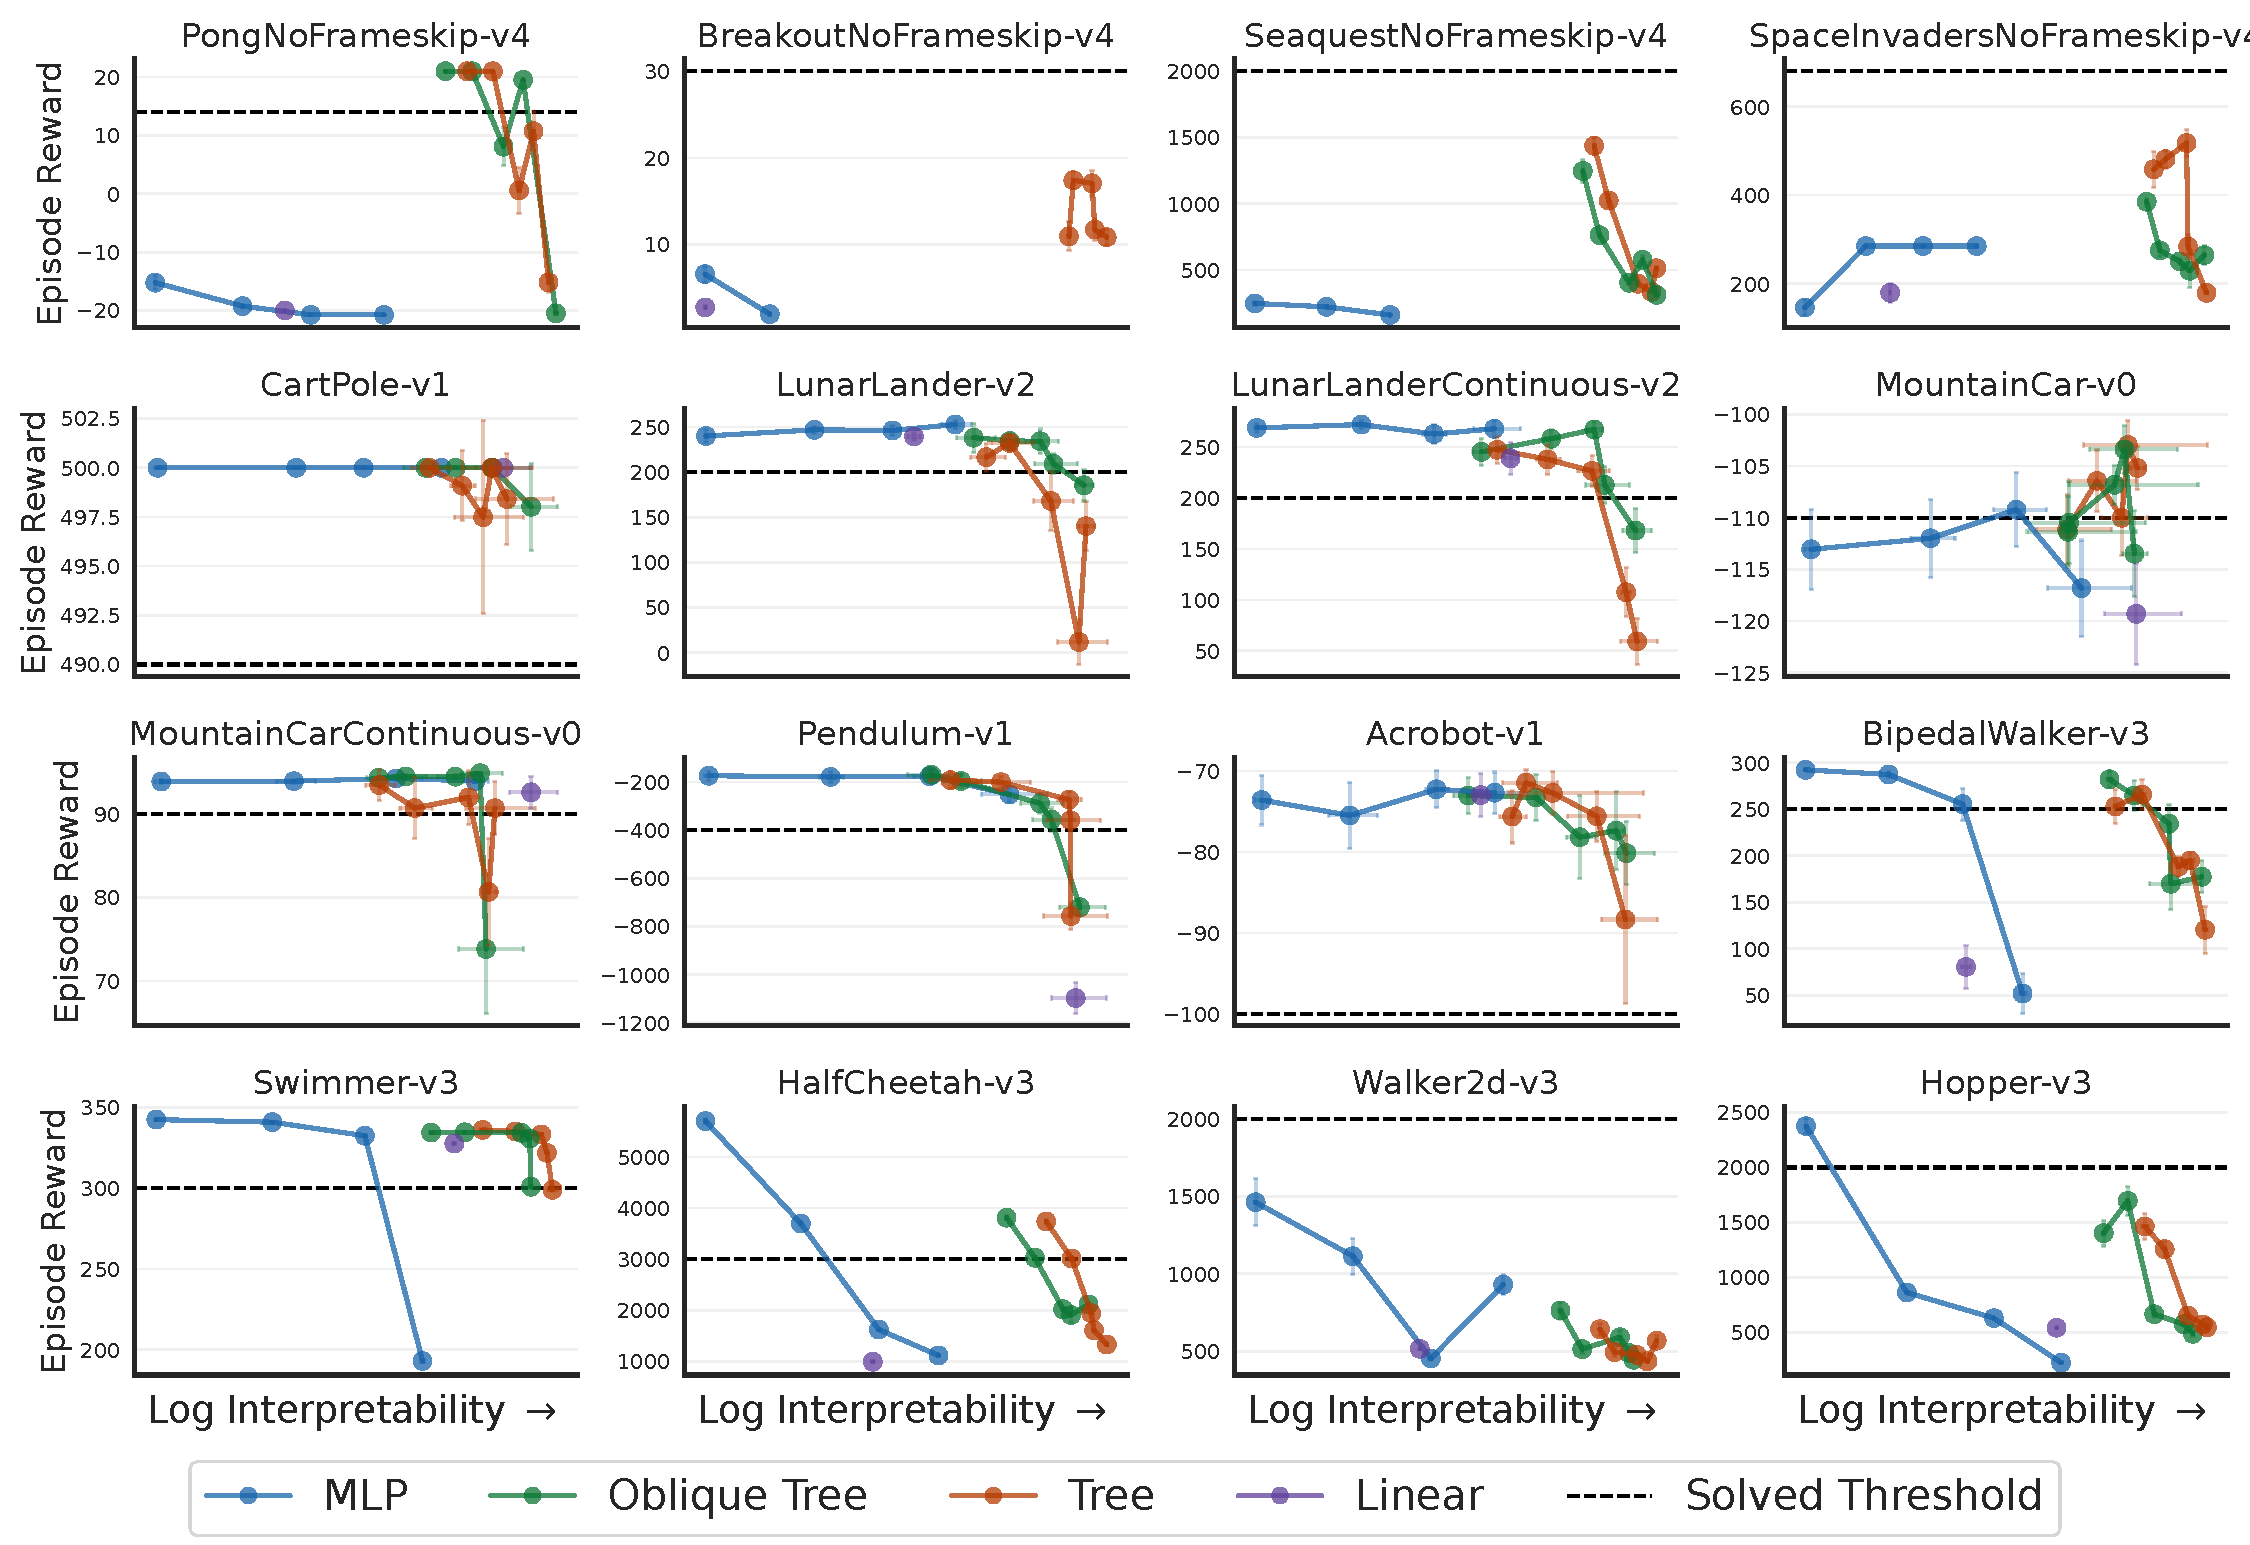
\includegraphics[width=1\linewidth]{images/images_part3/trade_off_step_times.pdf}
    \caption{Trade-off Cumulative Reward vs. Step Inference Time}
    \label{fig:trade-off}
\end{figure}

\begin{figure}[ht]
    \centering
    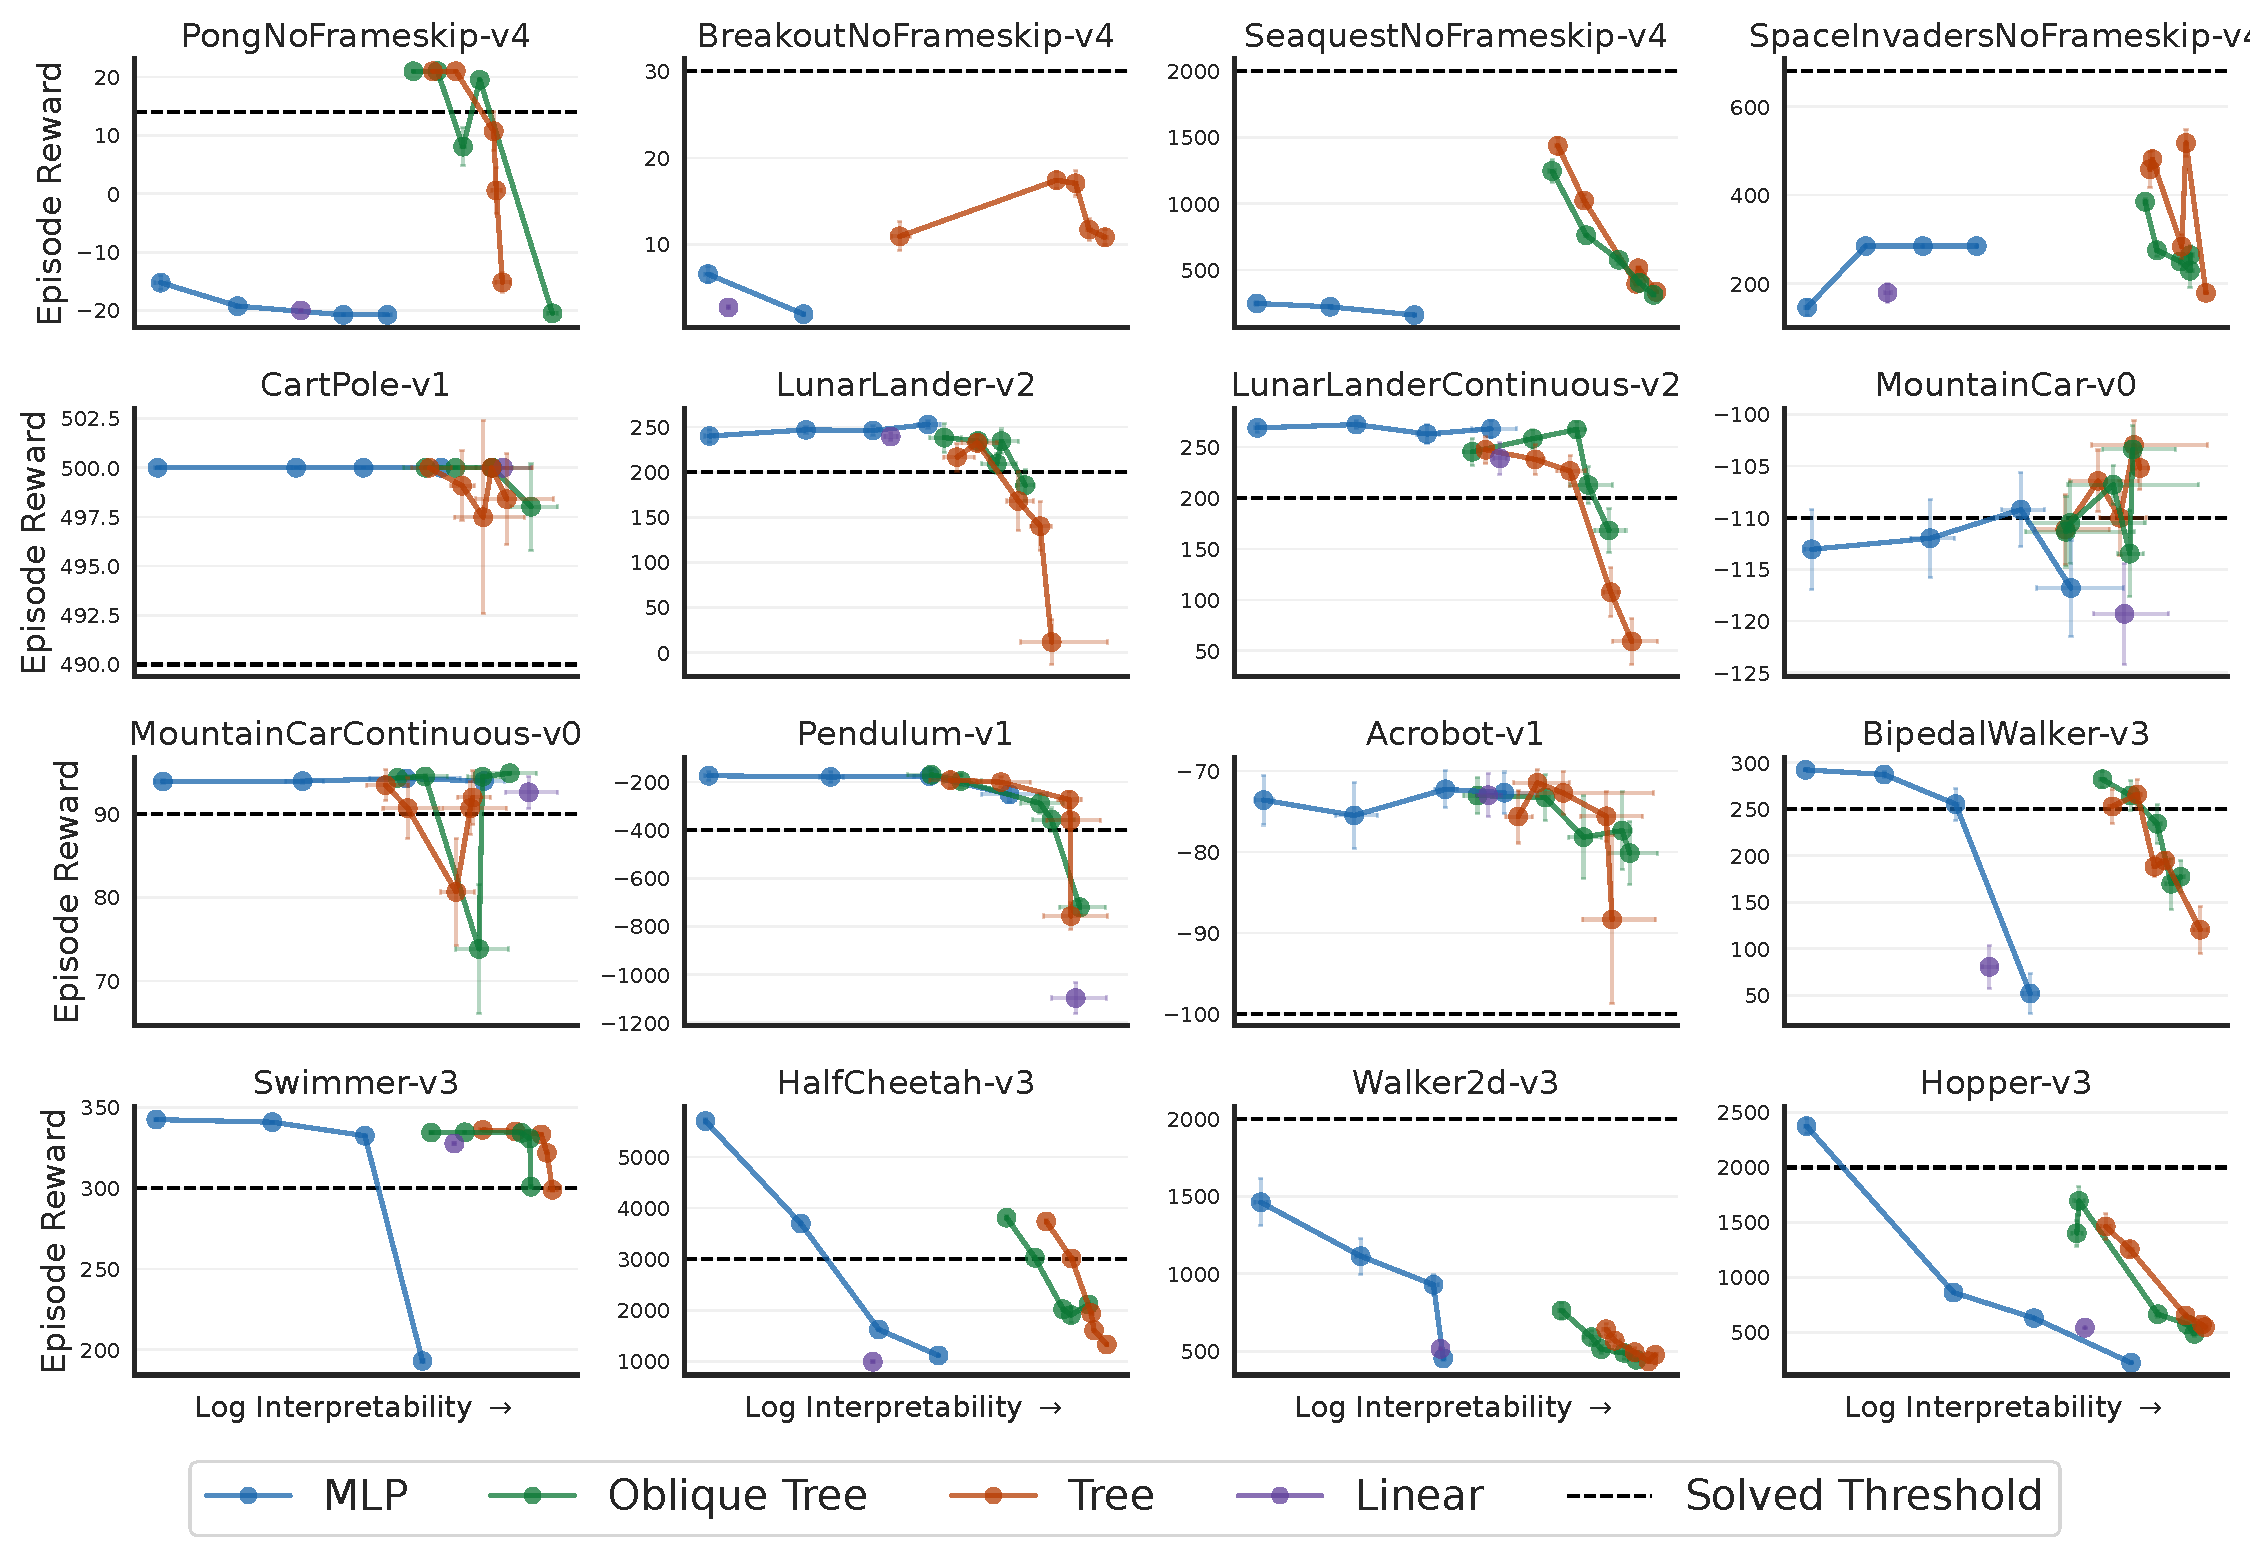
\includegraphics[width=0.95\linewidth]{images/images_part3/trade_off.pdf}
    \caption{Trade-off Cumulative Reward vs. Episode Inference Time}
    \label{fig:trade-off-episode}
\end{figure}

\begin{figure}[ht]
    \centering
    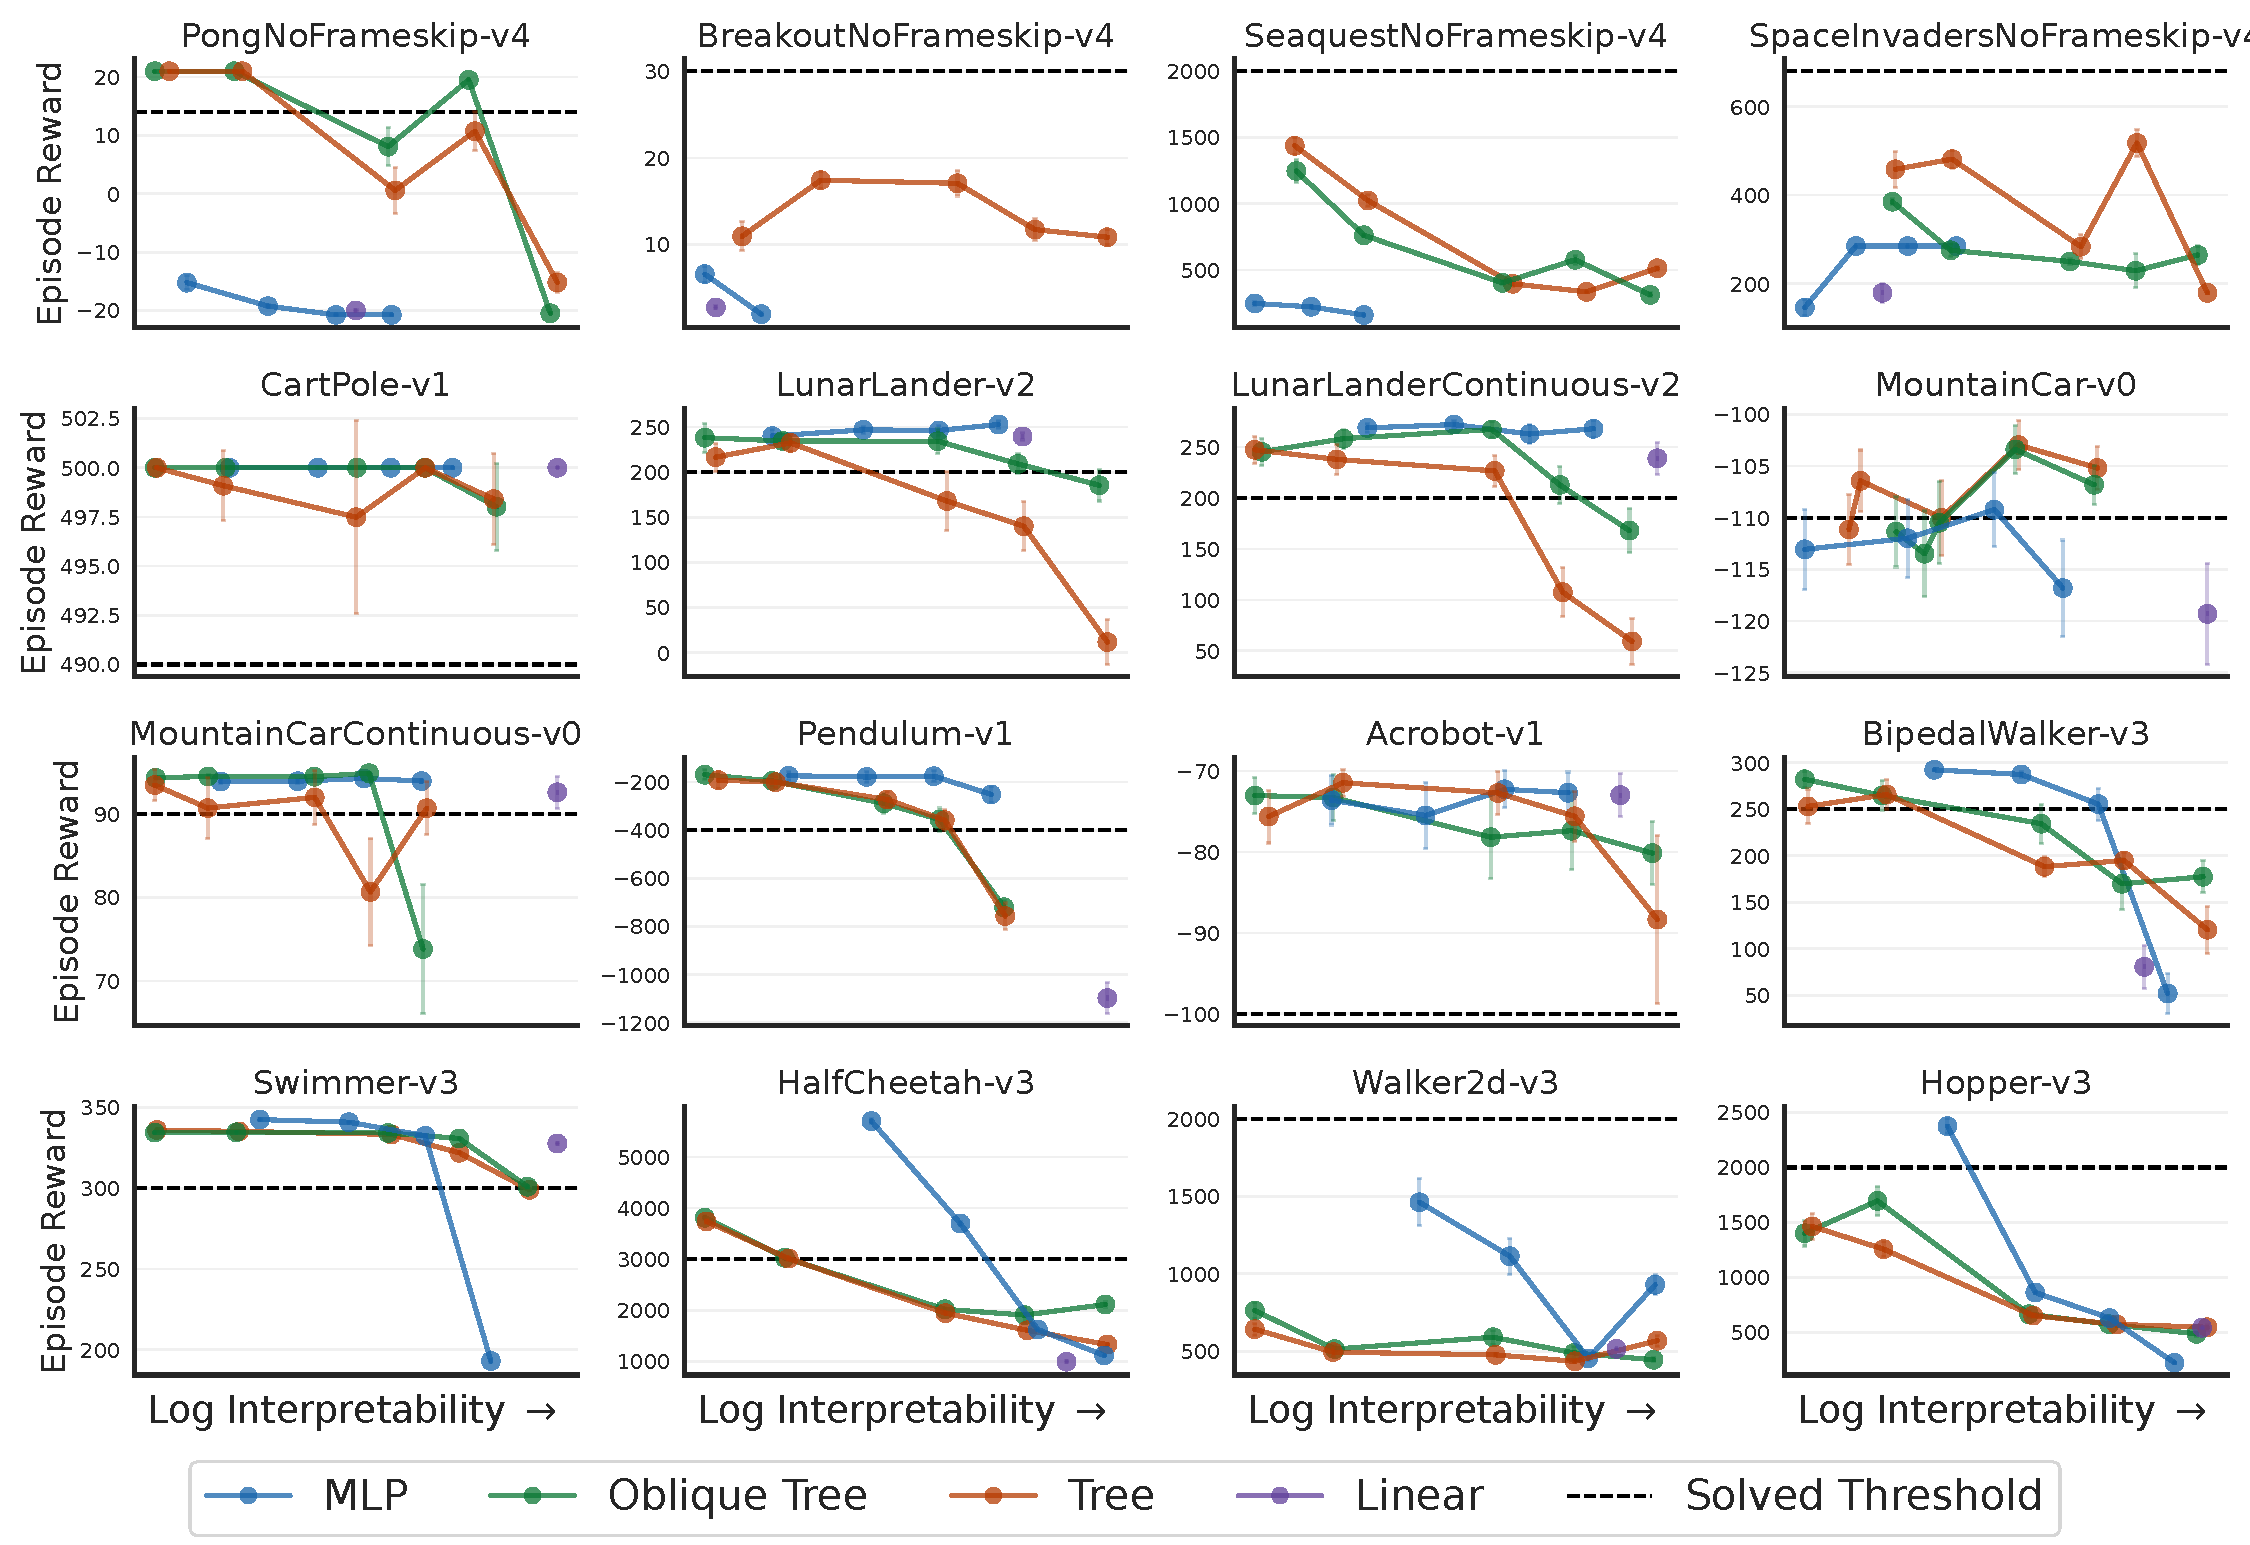
\includegraphics[width=0.95\linewidth]{images/images_part3/trade_off_size.pdf}
    \caption{Trade-off Cumulative Reward vs. Policy Size}
    \label{fig:trade-off-size}
\end{figure}